\documentclass[11pt,letterpaper]{article}
\usepackage[utf8]{inputenc}
\usepackage{amsmath}
\usepackage{amsfonts}
\usepackage{amssymb}
\usepackage{geometry}
\usepackage{hyperref}
\usepackage{xcolor}
\usepackage{booktabs}
\usepackage{caption}
\usepackage{float}
\usepackage{graphicx}
\graphicspath{{visual-assets/}}

% Brand Typography / Color configuration
\definecolor{mpdark}{HTML}{0F172A}
\definecolor{mpblue}{HTML}{3B82F6}
\definecolor{mpgreen}{HTML}{10B981}
\definecolor{mpred}{HTML}{EF4444}
\definecolor{mppurple}{HTML}{8B5CF6}
\definecolor{mpamber}{HTML}{F59E0B}
\definecolor{mpgrey}{HTML}{64748B}

\geometry{margin=1in}

\hypersetup{
    colorlinks=true,
    linkcolor=mpblue,
    urlcolor=mpblue
}

\setlength{\abovedisplayskip}{4pt}
\setlength{\belowdisplayskip}{4pt}
\setlength{\abovedisplayshortskip}{2pt}
\setlength{\belowdisplayshortskip}{2pt}

\newcommand{\plain}[1]{\par\smallskip\noindent\textcolor{mpgrey}{\textit{In plain terms:} #1}\par\smallskip}
\newcommand{\gap}{g}

\title{\vspace{-20pt}\textbf{\color{mpdark}Money Plot Labs Technical Whitepaper 006 \\
The Years-to-FI Surface: \\
Straight Contours, Sensitivities, and a Printable Model}}
\author{\textbf{Money Plot Labs}}
\date{October 2026}

\begin{document}

\maketitle

\begin{abstract}
\vspace{-5pt}
How many years until financial independence (FI), as a function of your income and your expenses? With a constant real return and an FI number set by a safe withdrawal rate, the answer has a closed form. Plotted over income and expenses, it becomes a surface. This paper derives that surface and the facts behind the FI Surface tool. First, a rewriting of the closed form that stays exact when savings are zero and when the return goes to zero. Second, a partition of the plane into \emph{already FI}, \emph{reachable} and \emph{never}. Third, the central result: every iso-year contour is a straight line, and all of them pass through a single focal point. So the years to FI depend only on the direction from that point. Fourth, analytic sensitivities, including an exact exchange rate between a dollar of spending and a dollar of income. Last, the method that turns the surface into a watertight, labeled 3D-printable model: constant-width raised lines, rasterized debossed text, and a closed mesh.
\end{abstract}

% =========================================================================
\section{The Model}
% =========================================================================

\begin{center}
\begin{tabular}{@{}ll@{}}
\toprule
$I$ & annual income, after tax \\
$X$ & annual expenses \\
$C = I - X$ & annual savings (negative if you spend more than you earn) \\
$R$ & real annual return ($R \ge 0$) \\
$S$ & safe withdrawal rate \\
$P_0$ & portfolio today \\
$F = X/S$ & FI number: the portfolio whose safe withdrawal covers your expenses \\
\bottomrule
\end{tabular}
\end{center}

All amounts are real (today's) dollars, as in the rest of the suite. Each year the portfolio earns $R$ and you add your savings:
\begin{equation}
P_n = P_{n-1}(1+R) + C \quad\Longrightarrow\quad P_n = P_0(1+R)^n + C\,s_n, \qquad s_n = \frac{(1+R)^n - 1}{R},
\label{eq:pn}
\end{equation}
where $s_n$ is the future value of \$1 saved per year for $n$ years ($s_n = n$ when $R = 0$). The years to FI are the $n$ at which $P_n = F$. Solving,
\begin{equation}
n = \frac{\ln\!\big( (F + C/R) \,/\, (P_0 + C/R) \big)}{\ln(1+R)}.
\label{eq:naive}
\end{equation}
Equation~\eqref{eq:naive} treats $n$ as continuous. At whole years it matches the recursion exactly. Between whole years it moves the crossing smoothly instead of in one-year steps. Figure~\ref{fig:timeline} shows the question in one picture. The portfolio grows from $P_0$, fed by savings and compounding. The FI number is a fixed line, and $n$ is where the two meet. Everything that follows is about how that meeting point moves as income $I$ and expenses $X$ change. Expenses move both the curve, through savings, and the line, through $F = X/S$.

\begin{figure}[H]
\centering
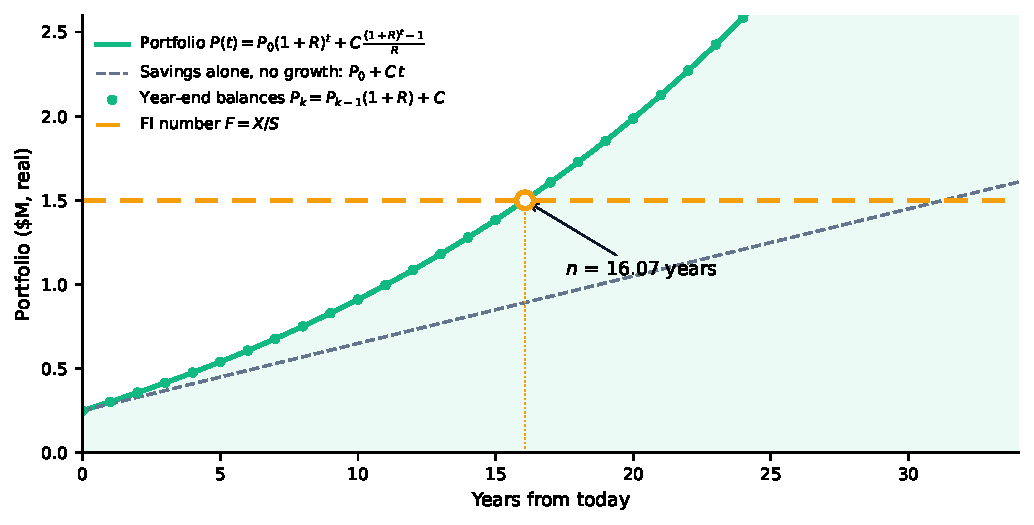
\includegraphics[width=0.85\textwidth]{fi_timeline.pdf}
\caption{What is solved for, for the reference household ($I = \$100$k, $X = \$60$k, $P_0 = \$250$k, $R = 5\%$, $S = 4\%$, age 35). The portfolio (green; dots are the year-end balances of the recursion) reaches the FI number $F = X/S = \$1.5$M after $n = 16.07$ years, at age 51. With savings alone and no growth it would take 31.25 years (dashed grey). The FI Surface tool draws this chart live as you change income and expenses.}
\label{fig:timeline}
\end{figure}

Whitepaper~001 solves a richer problem: a finite retirement horizon with a legacy floor. This paper keeps the simpler and widely used rule of thumb, ``FI when the portfolio reaches expenses $\div$ withdrawal rate.'' That simplification is what makes the geometry below exact.

\subsection{A form that never divides by zero}

Equation~\eqref{eq:naive} breaks down at $R = 0$ and is ill-conditioned when $C/R$ is large. Define
\begin{equation}
\gap = F - P_0 \quad\text{(how far you are from FI)}, \qquad u = R P_0 + C \quad\text{(the portfolio's growth in year one)}.
\end{equation}
Multiplying the numerator and denominator inside the logarithm of \eqref{eq:naive} by $R$ gives
\begin{equation}
\boxed{\,n = \frac{\ln\!\left(1 + R\gap/u\right)}{\ln(1+R)}\,}, \qquad \lim_{R \to 0} n = \frac{\gap}{u} = \frac{F - P_0}{C}.
\label{eq:n}
\end{equation}
This form is exact at $C = 0$, where it reduces to $\ln(F/P_0)/\ln(1+R)$, and it is continuous as $R \to 0$. It is also convenient to write $D = u + R\gap = C + RF$, so that $n = \ln(D/u)/\ln(1+R)$.

\plain{$u$ is how fast the pile is growing right now; $\gap$ is how far it still has to grow. The ratio $\gap/u$ would be the answer with no compounding, and the logarithm corrects for compounding.}

\subsection{Three regions}

Equation~\eqref{eq:n} is a finite, positive number exactly when $\gap > 0$ and $u > 0$. That splits the $(I, X)$ plane into three regions:
\begin{itemize}
\setlength\itemsep{1pt}
\item \textbf{Already FI}, $X \le S P_0$ ($\gap \le 0$): $n = 0$. The raw formula would return a negative ``time since FI'', which the tool reports as zero.
\item \textbf{Never}, $X \ge I + R P_0$ ($u \le 0$): spending eats all of the portfolio's growth, so the portfolio does not grow and never reaches $F$. Here $n = \infty$.
\item \textbf{Reachable}, everything else: $0 < n < \infty$.
\end{itemize}
The two boundaries are straight lines. One is horizontal at $X = SP_0$. The other has slope 1, offset by the portfolio's return $RP_0$.

\paragraph{Design note.} Plots and printed models need a finite height everywhere. The tool shows the never region, and everything beyond a cap $n_{\max}$, as a flat plateau at the cap. By default the cap follows the household's own $n$. It is the smallest of 20, 25, 30, 40, 50, 60 or 80 years that is at least $1.6n$ and $n + 5$ (past 30 years, $n + 15$), so their own point lies on the slope rather than in the plateau: 30 years for the reference household. Contours are drawn every 5, 10 or 20 years, three to six lines. The printed height of the cap is fixed, so a larger cap lowers the surface and shrinks the plateau rather than making the model taller. Mapping undefined values to \emph{zero} instead would draw a cliff that drops to the floor exactly where FI is hardest. That is the wrong message.

% =========================================================================
\section{Geometry: Straight Contours Through One Focal Point}
\label{sec:geometry}
% =========================================================================

Fix a number of years $L$. By \eqref{eq:pn}, $n = L$ means $F = P_0(1+R)^L + C\,s_L$:
\begin{equation}
\frac{X}{S} = (1+R)^L P_0 + s_L\,(I - X).
\end{equation}
This is \emph{linear} in $I$ and $X$, so every contour is a straight line:
\begin{equation}
X = X^\star + m_L\,(I - I^\star), \qquad m_L = \frac{S s_L}{1 + S s_L}, \qquad
\boxed{(I^\star, X^\star) = \big(P_0(S - R),\; S P_0\big)}.
\label{eq:contour}
\end{equation}
To check that every line passes through $(I^\star, X^\star)$, substitute: $X^\star(1/S + s_L) = P_0(1 + S s_L)$, and $(1+R)^L P_0 + s_L I^\star = P_0\big((1+R)^L + S s_L - R s_L\big) = P_0(1 + S s_L)$, using $R s_L = (1+R)^L - 1$.

The \textbf{focal point} has a direct meaning. At $X^\star = SP_0$ you are exactly at FI. At $I^\star = X^\star - RP_0$ your savings are exactly $-RP_0$: you spend precisely the portfolio's growth, so the portfolio never moves. The slope $m_L$ rises from $0$ at $L = 0$ (the horizontal ``already FI'' line) toward $1$ as $L \to \infty$ (the ``never'' line). Both boundaries of Section~1.2 pass through the focal point as well, so the reachable region is a wedge with its apex at $(I^\star, X^\star)$, and the contours fan out across it (Figure~\ref{fig:fan}).

Inverting $m_L$ gives the years to FI as a function of \emph{direction alone}:
\begin{equation}
n = \frac{\ln\!\big(1 + R\,s\big)}{\ln(1+R)}, \qquad s = \frac{m}{S(1-m)}, \qquad m = \frac{X - X^\star}{I - I^\star}.
\label{eq:angle}
\end{equation}

\plain{stand at the focal point and look into the wedge. Each direction you could look in corresponds to one number of years, and every income/expense pair along that line of sight takes the same time to reach FI. Raising income and spending together along that line changes nothing.}

When $R > S$, as in the reference case ($R = 5\%$, $S = 4\%$), the focal point sits at a negative income ($I^\star = -\$2{,}500$ for $P_0 = \$250$k). It lies just outside any realistic window, which is why the contours look like a fan opening from the left edge.

\begin{figure}[H]
\centering
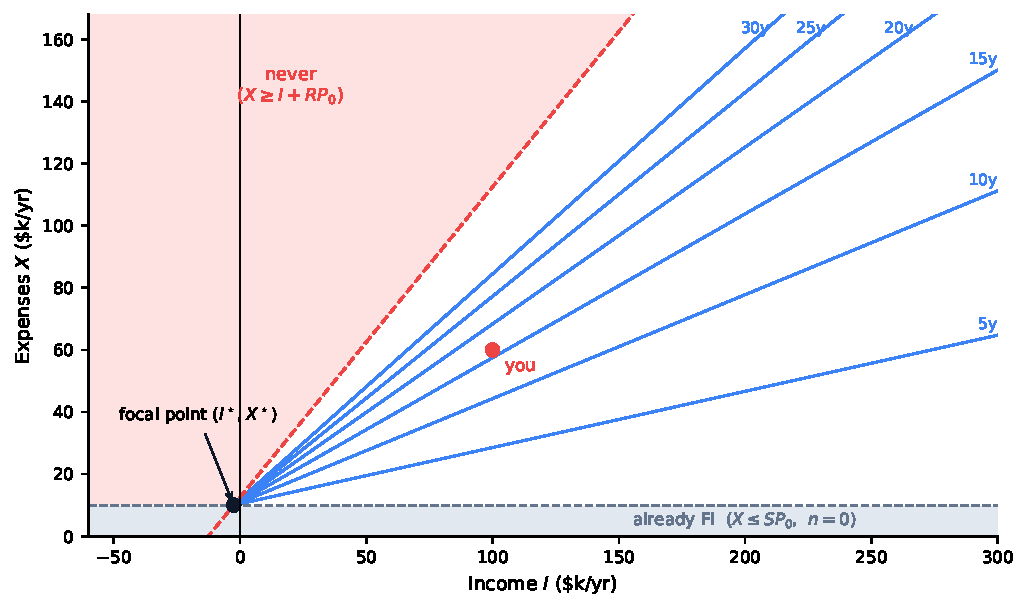
\includegraphics[width=0.85\textwidth]{fi_contour_fan.pdf}
\caption{The three regions and the iso-year contours for $R = 5\%$, $S = 4\%$, $P_0 = \$250$k. Every contour is a ray from the focal point $(I^\star, X^\star) = (-\$2.5\text{k}, \$10\text{k})$. The grey dashed line ($n = 0$) and the red dashed line ($n = \infty$) bound the reachable wedge.}
\label{fig:fan}
\end{figure}

\begin{figure}[H]
\centering
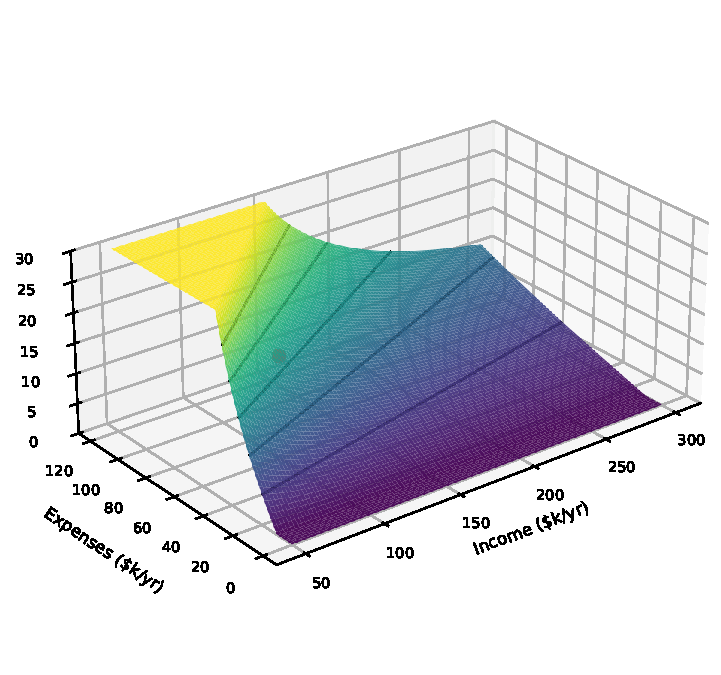
\includegraphics[width=0.7\textwidth]{fi_surface_3d.pdf}
\caption{The surface $n(I, X)$, capped at 30 years, with its 5-year contours. The red dot is the reference household ($I = \$100$k, $X = \$60$k): 16.07 years.}
\label{fig:surface}
\end{figure}

% =========================================================================
\section{Sensitivities}
\label{sec:sens}
% =========================================================================

Differentiating \eqref{eq:n}, with $\rho = R/\ln(1+R)$ ($\rho \to 1$ as $R \to 0$) and $D = u + R\gap$:
\begin{align}
\frac{\partial n}{\partial I} &= -\frac{\rho\,\gap}{u D}, &
\frac{\partial n}{\partial X} &= \frac{\rho}{D}\left(\frac{1}{S} + \frac{\gap}{u}\right), \\
\frac{\partial n}{\partial P_0} &= -\frac{\rho}{u}, &
\frac{\partial n}{\partial S} &= -\frac{\rho X}{S^2 D}, \\
\frac{\partial n}{\partial R} &= \frac{1}{\ln(1+R)}\left(\frac{F}{D} - \frac{P_0}{u} - \frac{n}{1+R}\right).
\end{align}

\paragraph{The exchange rate between spending and income.} By Section~\ref{sec:geometry}, $n$ is constant along rays from the focal point, so it is homogeneous of degree zero about $(I^\star, X^\star)$. Euler's theorem then gives $(I - I^\star)\,\partial_I n + (X - X^\star)\,\partial_X n = 0$:
\begin{equation}
\boxed{\;\frac{\partial n/\partial X}{-\,\partial n/\partial I} = \frac{I - I^\star}{X - X^\star} = 1 + \frac{u}{S\gap}\;}
\label{eq:exchange}
\end{equation}
The ratio always exceeds 1. A dollar of spending cuts savings exactly as a dollar of lost income does, \emph{and} it raises the FI number by $1/S$ dollars. The ratio is largest close to FI: as $\gap \to 0$, cutting spending is worth far more than earning more.

\plain{for the reference household, spending \$1 less per year does as much as earning \$2.05 more.}

\begin{figure}[H]
\centering
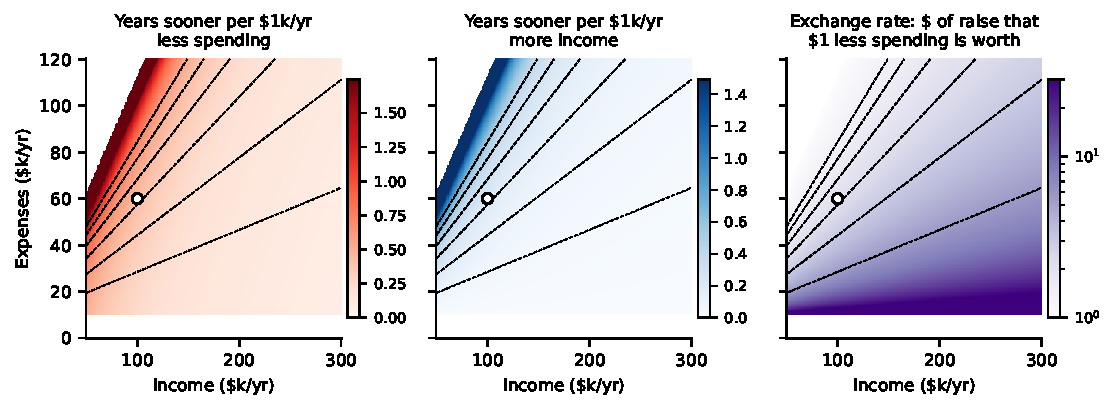
\includegraphics[width=\textwidth]{fi_sensitivity.pdf}
\caption{Years sooner per \$1k/yr less spending (left) and per \$1k/yr more income (center), and the exchange rate \eqref{eq:exchange} between them (right, log scale). Dashed: 5-year contours. Blank: already FI.}
\label{fig:sens}
\end{figure}

\subsection{Worked example}

For the tool's defaults, $I = \$100$k, $X = \$60$k, $P_0 = \$250$k, $R = 5\%$, $S = 4\%$:

\begin{center}
\begin{tabular}{@{}lr@{}}
\toprule
FI number $F = X/S$ & \$1{,}500{,}000 \\
Gap $\gap = F - P_0$ & \$1{,}250{,}000 \\
Year-one growth $u = RP_0 + C$ & \$52{,}500 \\
$D = C + RF$ & \$115{,}000 \\
Years to FI $n$ & 16.07 \\
\midrule
\$1k/yr less spending & 0.435 years sooner \\
\$1k/yr more income & 0.212 years sooner \\
Exchange rate \eqref{eq:exchange} & 2.05 \\
+1 point of real return ($100\cdot\partial n/\partial R$) & 1.440 years sooner \\
+\$100k portfolio today & 1.952 years sooner \\
+0.1 point withdrawal rate & 0.334 years sooner \\
\bottomrule
\end{tabular}
\end{center}
The tool's ``+1\% Real Return'' card uses a centered difference over $R \pm 0.5\%$ (1.444 years). That differs from the derivative only by the curvature in $R$.

% =========================================================================
\section{From Surface to Solid}
\label{sec:print}
% =========================================================================

The tool, and its companion Python notebook, turn the surface into a 3D-printable STL. Every step is deterministic and runs in the browser.

\subsection{Heightmap}

The model is a heightmap $z_{ij}$ on a regular grid with cell size $c$ (0.25~mm by default for the STL; the tool's on-screen preview uses 0.35~mm). The plot area maps income and expenses linearly at a scale $\sigma$ in millimeters per \$10k/yr, the same on both axes by default. The tool fits the window and the scale to the household. Incomes run from about a third of theirs to twice it (at least \$100k above it). Expenses run from \$0 to twice theirs or 80\% of their income, whichever is more. Both are rounded to grid steps that give at most eight ticks. $\sigma$ is then the largest half-millimeter for which the whole model fits a $225 \times 150$~mm footprint. For the reference household that is incomes \$25k--\$200k, expenses \$0--\$120k, and 10~mm per \$10k: a $175 \times 120$~mm plot, $202 \times 147$~mm with its ledges (sized for a 0.6~mm nozzle, below). With one scale, a dollar of income and a dollar of spending are the same distance apart. A contour's slope on the model then is its real exchange rate, and the 45$^\circ$ never line looks like 45$^\circ$. It is surrounded by flat \emph{ledges} that carry the text, each sized to fit the text on it (18~mm front and left and 9~mm back and right at the default text sizes). Heights are
\begin{equation}
z = \begin{cases}
b & \text{on the ledges}, \\
b + \ell + \min(n, n_{\max})\,H/n_{\max} & \text{on the plot},
\end{cases}
\end{equation}
where $b$ is the base thickness (2.4~mm), $\ell = 1$~mm lifts the plot so its edge reads as a step, and $H$ is the height at the cap (60~mm).

\paragraph{Slicer layers.} A printer builds the model in layers of height $\lambda$ above a first layer $\lambda_1$ (0.2~mm each by default), so a horizontal feature prints cleanly only when it lies on a layer boundary $\lambda_1 + k\lambda$. The base $b$, the top of the plot step $b + \ell$, the text depth and every contour top (below) are rounded to the nearest boundary.

\subsection{Raised lines with a constant printed width}

Each raised line has a width $w$, a height $h$ and a top $\tau(\mathbf x)$. Every grid point within $w/2$ of the line, measured as the distance $d$ in millimeters, is raised to the top:
\begin{equation}
z \leftarrow \max\big(z,\; \tau(\mathbf x)\big) \quad\text{where } |d| \le w/2 .
\end{equation}
The edges are sharp. A soft, anti-aliased edge would leave in-between heights, and those slice into stray specks. Overlapping lines combine with $\max$, so crossings don't stack.

\paragraph{Contours are level, and start on their line.} Along an iso-year line the surface height is constant, $z_L = b + \ell + L\,H/n_{\max}$, rounded to a layer boundary. So a contour's shape is level. Every shape lies on the \emph{uphill} side of its line ($-w \le d \le 0$, where $d < 0$ means more years), so its downhill edge is the line itself. Three shapes are offered:
\begin{itemize}
\setlength\itemsep{1pt}
\item \textbf{step:} a cliff rising from the line, from $z_L$ to a flat top $\tau = z_L + h$, also on a layer boundary. You can feel it, and it reads in one color.
\item \textbf{shelf:} a level notch cut into the slope at exactly $z_L$, $w$ wide. Its floor is one layer at the line's own height, so an accent color there makes an even line whose downhill edge is the true contour.
\item \textbf{none:} no shape. A color change at $z_L$ already traces the iso-year line exactly, wherever the surface crosses that height.
\end{itemize}
The obvious alternative, raising the surface by $h$ along a band centered on the line, has two faults. Its top tilts with the slope, by about $|\nabla z|\,w$: some 1.7~mm, or eight 0.2~mm layers, across a 1.2~mm ridge where the surface is steep. The slicer then cuts that tilted strip into slivers on every layer. And its edges sit $w/2$ either side of the line instead of on it.

\paragraph{A step is filled to the slope.} Uphill of a step, the surface climbs back to its top only at a distance $h/|\nabla z|$ from the line. That is 0.2--3.3~mm on the default model, widest on the gentle part of the 5-year line. In between, the surface lies below the top. So the top layer would also appear a second time, a little uphill, where the slope reaches the same height: a false line at about $L + h\,n_{\max}/H$ years. The step's level top is therefore extended uphill, up to 8~mm, until it meets the slope. The top layer is then one continuous band from the line to where it meets the slope, wider where the slope is gentle. (A horizontal layer of thickness $t$ on a slope $s$ always shows as a band $t/s$ wide; that is why an even accent line needs the shelf.) The contour at the cap borders the flat plateau, which never climbs back to the top, so it gets no fill.

\paragraph{Lines that climb.} Your income and expense lines and the grid lines run up the slope, so they cannot be level. Their top follows the surface along the line and is level across it: for the line $x = x_0$, $\tau(x, y) = z(x_0, y) + h$, and likewise for $y = y_0$. \paragraph{A flat plateau.} Nothing rises above the cap height $b + \ell + H$. Your lines and the grid mean nothing past the cap, so where they run into the plateau they level off into it, and a step on the cap contour adds no rim. The plateau stays one flat top for the whole region of $n_{\max}$ or more years, including never. \paragraph{Your dot.} Where your two lines cross, the web tool adds a raised disc, 8~mm across, with vertical walls and a level top on a layer boundary 3~mm above the highest surface beneath it, so your own point stands out from the grid by sight and by touch. It is traced like a contour shape (its field is $r - \lVert (x, y) - (x_Y, y_Y) \rVert$), labels keep clear of it, and it is the one feature allowed above the plateau (when you are on it).

The sizes depend on the nozzle. Every line, and every letter stroke and gap (about $0.15\times$ the text size), should be at least two extrusion lines wide. For a 0.6~mm nozzle (the default): contour shapes $w = 1.4$~mm, your own income and expenses $1.8$~mm, grid lines $1.2$~mm, and text 6~mm on the ticks, 6.5~mm for titles and 5.5~mm beside the lines. For a 0.4~mm nozzle these become 1.2, 1.6 and 0.8~mm and 5, 5.5 and 4.5~mm. A step is $h = 1.0$~mm high, your lines 1.4~mm and the grid 0.5~mm.

A simpler alternative marks a contour wherever $|n - L| < \delta$. Its printed width is $2\delta/|\nabla n|$, which is a hairline where the surface is steep and a smear where it is flat (Figure~\ref{fig:ridge}). Because contours are straight rays from the focal point, \eqref{eq:contour} gives the exact distance instead. With the ray's unit direction $\hat u$ in millimeter coordinates and the focal point at $\mathbf f$:
\begin{equation}
d = (\mathbf{x} - \mathbf{f}) \times \hat u \quad \text{where } (\mathbf{x} - \mathbf{f})\cdot \hat u > 0, \qquad d = \infty \text{ elsewhere}.
\end{equation}
The first-order estimate $|n - L|/|\nabla n|$ would do nearly as well, except near the never line. There $|\nabla n| \to \infty$ faster than $n$ grows, and the estimate draws a spurious ridge.

\begin{figure}[H]
\centering
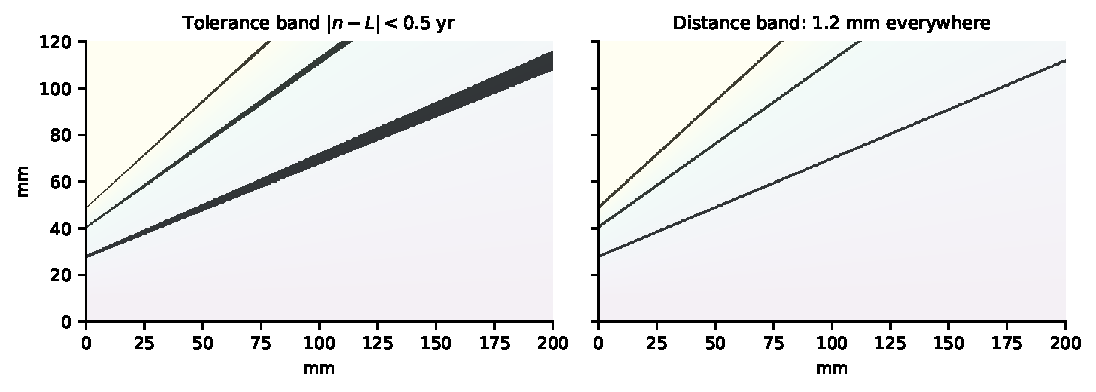
\includegraphics[width=0.95\textwidth]{fi_ridge_width.pdf}
\caption{The 10-, 20- and 30-year contour ridges on a $200 \times 120$~mm plot. Left: a tolerance band in years is thick where the surface is flat and nearly vanishes where it is steep. Right: the distance band prints 1.2~mm wide everywhere.}
\label{fig:ridge}
\end{figure}

\subsection{Labels: debossed or embossed text}

Text is rasterized (4$\times$ supersampled) into the fraction $\kappa$ of each grid \emph{cell} it covers. Averaging the four cells around each grid point gives a field $\phi_{ij}$: the text blurred by a box two cells wide. Letters are where $\phi \ge \tfrac12$. For a straight edge, $\phi$ ramps linearly across both grid points beside it and crosses $\tfrac12$ exactly on the edge. That holds for any stroke at least one cell wide. So interpolating along each grid edge puts the outline where the letter really is, inside the cell rather than on the grid (Section~\ref{sec:mesh}). Letters are cut in (deboss) or raised (emboss) by a depth $t$ (0.6~mm, a whole number of layers), with \emph{vertical} walls and a floor parallel to the surface.

Both properties matter for printing. The obvious alternative subtracts $t\kappa$ from the heightmap, giving partial depths along the letter edges. Each wall then leans across at least a full cell, because every heightmap triangle spans one, and the anti-aliased band adds another. A 0.8~mm stroke becomes a V-shaped groove about 1.4~mm wide at the top. A slicer cuts that groove at a different width on every layer, so the layers of each letter no longer sit on top of one another. A plain per-cell mask fixes the walls but stair-steps every curve at the cell size. Traced outlines with vertical walls give both clean layers and smooth letters.

The ledge text is configurable: the two axis titles, the caption (by default ``OCT 2026 $\cdot$ \$250k SAVED $\cdot$ 5\% RETURN $\cdot$ 4\% SWR'': the month names whose dollars the real amounts are in, and it shrinks to fit beside the title, or moves to the back ledge), the prefix on the ``you'' labels, an optional small site address (on the right ledge, else the back), whether tick labels are shown, and every text size. An empty title is dropped, and the ledges resize to fit what remains. Placement:
\begin{itemize}
\setlength\itemsep{1pt}
\item \textbf{Ledges:} the tick labels sit centered under (or beside) each grid line, and the axis titles and a caption with the month, $P_0$, $R$ and $S$ sit outside them. A label at the end of an axis slides inward only when it would leave the model. One that would still overlap its neighbor is dropped.
\item \textbf{Inline:} each raised contour and each ``you'' line gets a label that runs along it (the angle is folded into $(-90^\circ, 90^\circ]$ so text never reads upside down). It is offset just clear of the line. Candidate positions are sampled along the line: on both sides for a ``you'' line, but only the uphill side for a contour. A contour's label then sits inside the band of years that starts at its line, so with year bands each band carries exactly one label, its own starting year. A candidate is rejected if its rotated box leaves the plot, touches a contour or ``you'' ridge (with a 0.8~mm gap), or touches another label (1~mm gap). Among the rest, the label goes where the cost
\[ \max_{\text{box}} |\nabla z| \;+\; 2 \times (\text{fraction of the box on a grid ridge}) \]
is lowest. That is the flattest free stretch, where debossed text prints cleanest.
\item \textbf{Fallback:} contours bunch together near the never line. A contour with no room for an inline label is labeled on the back or right ledge, where it leaves the plot.
\end{itemize}

\subsection{A watertight mesh}
\label{sec:mesh}

The solid is meshed directly from the heightmap. With an $n_x \times n_y$ grid and $B = 2(n_x - 1) + 2(n_y - 1)$ boundary edges:
\begin{itemize}
\setlength\itemsep{1pt}
\item \textbf{top:} two triangles per cell, wound counter-clockwise seen from above (normals up);
\item \textbf{walls:} two triangles under each boundary edge, down to $z = 0$, facing out;
\item \textbf{bottom:} a single fan of $B$ triangles from one center vertex to a copy of the boundary loop at $z = 0$, facing down. The flat base costs $B$ triangles rather than $2(n_x - 1)(n_y - 1)$;
\item \textbf{text:} every grid point inside a letter ($\phi \ge \tfrac12$) gets a second vertex at $z \pm t$. Every grid edge whose ends disagree gets a crossing point, at $\phi = \tfrac12$ by linear interpolation (kept 5\% off the corners), with a surface vertex and a letter vertex. A cell with mixed corners is split marching-squares style: walk its outline counter-clockwise through the corners and crossings, take the letter side and the surface side as separate convex polygons, and fan each. A saddle cell, where two opposite corners are inside, joins whichever side holds the cell's average. Each chord where the outline crosses the cell gets a vertical wall of two triangles. The wall runs along the reverse of that chord in both pieces, which keeps the orientation consistent for deboss and emboss. Grid points on the outer edge are never inside, so the model's sides stay plain.
\item \textbf{contour shapes:} shelves and steps are the same kind of feature, a second layer with vertical walls, using the signed distance inside the shape as their field (for a shelf $\min(-d,\, d + w)$, which is $\tfrac12$ exactly on both edge lines once offset by $\tfrac12$) and their own height for the layer: a shelf's floor $z_L$ or a step's top $\tau_L$. Their edges are straight lines at any angle to the grid. Traced this way they print as clean lines rather than a zig-zag of grid cells, and a test confirms every traced crossing lies on its exact line (to within the 5\% corner margin). At a crossing the shape's layer keeps the shape's own height (not one interpolated toward the neighboring surface), so both walls are truly vertical. Where a wall would have no height, as on a shelf's edge at its own line or where a step's top meets the slope, its two vertices are merged, so the mesh carries no zero-area facets for the slicer to repair. Letters never touch a contour shape: labels keep clear of them.
\end{itemize}
Without text that is $V = n_x n_y + B + 1$ vertices and $T = 2(n_x - 1)(n_y - 1) + 3B$ triangles. Text adds one vertex per copied grid point, two per outline crossing, and at most eight triangles per cut cell. Every edge is shared by exactly two triangles with opposite orientation, so the surface is closed and consistently oriented. Text only adds pockets or bumps to that surface, so the Euler characteristic stays $V - E + T = 2$ with $E = 3T/2$. The signed volume $\frac16\sum \mathbf a\cdot(\mathbf b \times \mathbf c)$ is positive. The binary STL takes $84 + 50T$ bytes: about 45~MB at 0.25~mm, 25~MB at 0.35~mm and 120~MB at 0.15~mm for the default model. Print it flat with no supports.

\subsection{Colors from layers}

A printer with one nozzle can change filament only between layers, so color is a function of height. On this model height \emph{is} years to FI. A color change at the height of contour $L$ therefore follows exactly the iso-year line, wherever it runs across the surface. The tool lists the swaps by layer, each $z$ being the top of the first layer printed in the new color:
\begin{itemize}
\setlength\itemsep{1pt}
\item \textbf{accent lines:} the accent goes on one layer per contour, swapping in at the layer ending at that height and back one layer later. With a shelf (the tool's default for this mode), that layer is the shelf's floor at $z_L$: an even line, $w$ wide, whose downhill edge is the contour. With a step, it is the step's top at $\tau_L$: a band from the line to where the top meets the slope.
\item \textbf{year bands:} alternating colors, starting one layer above each line's height $z_L$, shade each band of years in its own color. The color boundary is exactly the iso-year line, so no shape is needed (the default for this mode). With a step, the boundary falls at the foot of its cliff, which is again the line.
\item \textbf{base labels:} printing in the accent up to the letter floors ($b - t$) and switching just above them colors every debossed ledge letter. Labels on the surface sit at many heights and take whatever color their layer has.
\end{itemize}
The plateau's top layer is the cap contour's layer. So in line mode the whole $n_{\max}$+ region takes the accent, and in band mode it gets its own band, starting on that layer. No swap is listed above the model's last layer. The side walls show each swap as a horizontal stripe at its height: a scale of years up the side of the model.

\begin{figure}[H]
\centering
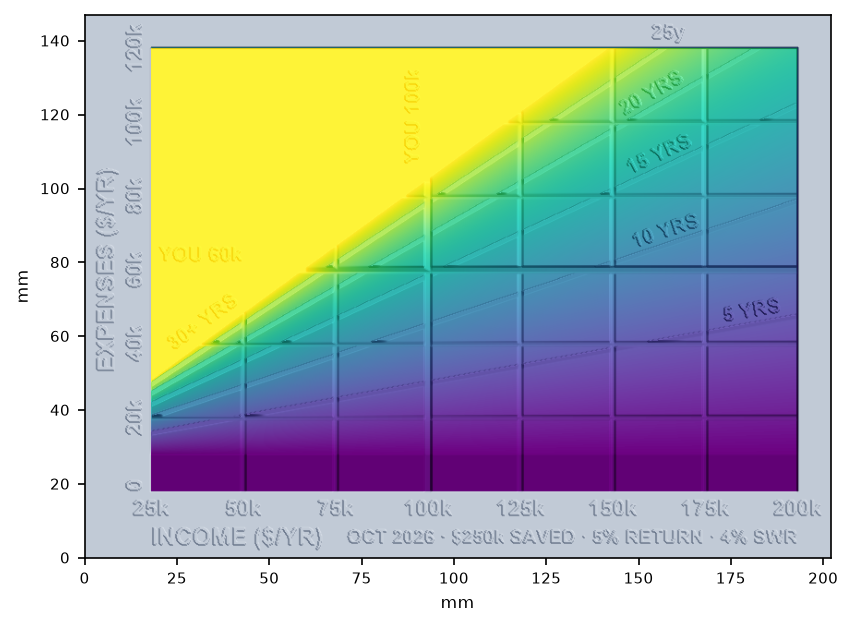
\includegraphics[width=0.88\textwidth]{fi_print_preview.png}
\caption{The default print model (hillshaded top view at 0.25~mm). It has debossed tick labels and axis titles on the ledges, an inline label beside each contour and ``you'' line (where a contour has no room inline, its label moves to the back or right ledge), and a flat plateau for 30+ years.}
\label{fig:print}
\end{figure}

% =========================================================================
\section{Validation}
% =========================================================================

The engine (\texttt{fisurface-engine.js}) is unit-tested under Node, and the notebook runs the same checks:
\begin{itemize}
\setlength\itemsep{1pt}
\item \eqref{eq:n} against the year-by-year recursion \eqref{eq:pn}, at 500 random $(I, X)$: exact at whole years and within one year between them. Infinite exactly where the recursion never crosses.
\item Every point on the line \eqref{eq:contour} has $n = L$ to $10^{-9}$; the $R \to 0$ limit and the $C = 0$ case match their closed forms.
\item The analytic partials match centered finite differences, and the Euler identity behind \eqref{eq:exchange} holds to machine precision.
\item The print model: ledge and surface heights; a raised line at its top across exactly its width, with no in-between heights; every contour level, with a single top on a layer boundary; base, step and text depth in whole layers; every label placed at the defaults, no two labels overlapping (separating-axis test), and no text upside down.
\item The mesh: every directed edge appears once and its reverse once (closed and consistently oriented), the volume of a flat slab is exact, and the STL layout is standard. With text cut or raised, the mesh is still closed, including random fields that exercise every saddle case. A round letter changes the volume by its area $\times\, t$ to within 1\%. Every vertex lies on the surface, at the surface $\pm t$, or on the bottom, so the text walls are vertical. A straight letter edge is traced at its true position, to within the test's sampling step. Every contour is level, with a single top on a layer boundary, and the color plan's swaps land on layer boundaries.
\end{itemize}

% =========================================================================
\section{Limitations}
% =========================================================================

The surface inherits every simplification of its model. It assumes a constant real return (the Stress Tester, Whitepaper~003, covers sequence risk), constant income and spending, no taxes on withdrawals, and a fixed withdrawal-rate definition of FI that ignores the length of retirement (Whitepaper~001 handles a finite horizon). Fractional years interpolate between annual steps. Treat the surface as a map of \emph{relative} effects: how much each lever moves the date, and how the levers trade against each other. Do not treat it as a forecast of the date itself.

\end{document}
